%%%%%%%%%%%%%%%%%%%%%%%%%%%%%%%%%%%%%%%%%%%%%%%%%%%%%%%%%%%

\chapter{Introduzione}
\label{chap:Introduzione}

%%%%%%%%%%%%%%%%%%%%%%%%%%%%%%%%%%%%%%%%%%%%%%%%%%%%%%%%%%%

\section{Contesto applicativo}
\label{sec:intro1}

Ciao ragazzi :D questo è un template che potete utilizzare per scrivere la vostra tesi in \LaTeX (sì, il nome di questo linguaggio è tutto un programma...)

Cos'è \LaTeX ? Cercatevelo su Wikipedia\footnote{http://it.wikipedia.org/wiki/LaTeX}!

A parte gli scherzi... è un linguaggio che vi permette (in poche parole) di creare documenti accademici (e non) con uno stile molto professionale. Gran parte del lavoro sporco (creazione dei capitoli, delle sezioni, dell'indice, della bibliografia, gestione dei margini, ecc...) viene interamente gestito da \LaTeX , le poche cose da configurare sono già state impostate in questo template... (quindi in poche parole avete già tutto pronto, stronzi!)

In questo pdf è spiegato un po' come far funzionare il tutto, ovvero:
\begin{itemize}
\item Dove scaricare l'IDE e come configurarlo
\item Come scaricare il compilatore
\item Come iniziare a personalizzare questo template
\end{itemize}

Cercherò di utilizzare più elementi \LaTeX possibile nello scrivere questa guida (tabelle, elenchi puntati, footnote, immagini...) così quando andrete a leggere il codice vi imparate pure qualcosa, caproni (<3)

%%%%%%%%%%%%%%%%%%%%%%%%%%%%%%%%%%%%%%%%%%%%%%%%%%%%%%%%%%%

\section{Motivazioni e obiettivi}
\label{sec:intro2}

Il principale motivo che mi spinge a creare questo pdf è quello di risparmiarvi gran parte delle rotture che si trovano quando ci si avvicina al mondo \LaTeX... insomma mi auguro che questa guida vi permetta di avere un buon punto d'inizio.

Come già spiegato nella sezione precedente, \LaTeX offre tantissimi servizi utili ed uno stile professionale unico, cose che su altri programmi (come Microsoft Word) potete anche sognarvi.

Insomma... con \LaTeX potete presentare una tesi fatta come si deve :)

%%%%%%%%%%%%%%%%%%%%%%%%%%%%%%%%%%%%%%%%%%%%%%%%%%%%%%%%%%%

\section{Risultati raggiunti}
\label{sec:intro3}

Nella Figura \ref{fig:latexVsWord} potete ammirare quanto \LaTeX sia più figo di Microsoft Word, ooooooh...

\begin{figure}[h] %La "h" indica che la figura si posizionerà "here". Usate "t" per "top" e "b" per "bottom"
\centering %centrata
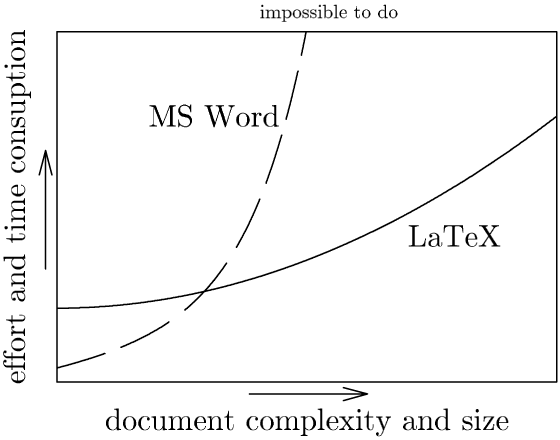
\includegraphics[width=0.8\linewidth]{latexVsWord} %larghezza e nome del file
\caption{Oooooooh che figo \LaTeX, ooooooooh} %didascalia
\label{fig:latexVsWord} %label per il riferimento
\end{figure}

%%%%%%%%%%%%%%%%%%%%%%%%%%%%%%%%%%%%%%%%%%%%%%%%%%%%%%%%%%%

\section{Organizzazione della tesi}
\label{sec:intro4}

Vi spiego brevemente quali sono le parti di questo template:

\begin{description}
  \item[Susanna.tex] Questo è il file principale del template: contiene le impostazioni generali e la struttura della tesi. Ricordate di impostarlo come documento master ogni volta che iniziate a lavorare alla tesi (ovviamente potete rinominarlo, nabbazzi)
  \item[frontespizio.tex] Sarebbe la copertina della tesi, nonchè la prima pagina. Contiene nome dell'università, del dipartimento, nome della tesi bla bla bla... io ho scelto un argomento di Fisica molto importante <3
  \item[dedica.tex] Una pagina dove scrivete a chi dedicate la tesi (Susanna <3)
  \item[introduzione.tex] Il file che contiene questo capitolo introduttivo (vi consiglio di creare appunto un file .tex per ogni capitolo). Le 4 sezioni di questo capitolo (\nameref{sec:intro1}, \nameref{sec:intro2}, \nameref{sec:intro3} e \nameref{sec:intro4}) sono le 4 sezioni standard da inserire nell'introduzione di una tesi, quindi vi consiglio di lasciarle così
  \item[start.tex] Contiene l'unico capitolo utile di questo documento: spiega come scaricare l'occorrente e come configurare il tutto per lavorare con \LaTeX
  \item[conclusione.tex] Contiene la conclusione (YOU DON'T SAY)
  \item[bibliografia.bib] Contiene i dati relativi alle fonti che citerete nella tesi (ad esempio, ora sto citando un libro sugli algoritmi genetici \cite{5635176}, l'unico inserito nella bibliografia di questo template)
  \item[IEEEtran.bst] È lo stile della bibliografia, non lo toccate
  \item[imgs] Cartella contenente le immagini (YOU DON'T SAY AGAIN)
\end{description}

